\documentclass{standalone}
\usepackage{pgfplots}
\pgfplotsset{compat=newest}
\begin{document}
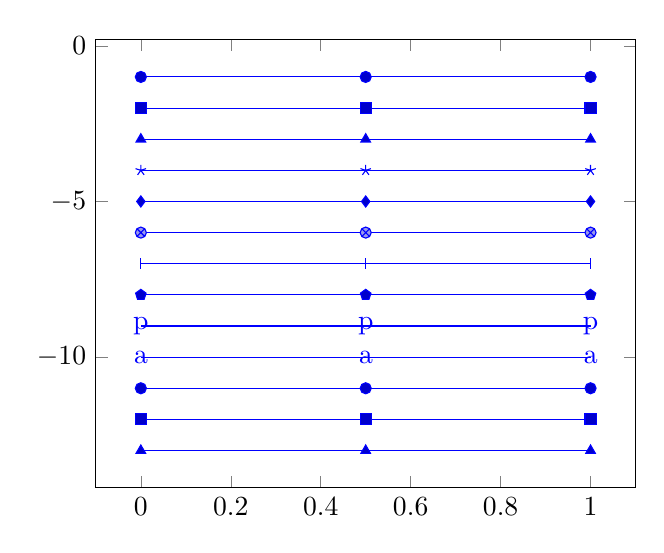
\begin{tikzpicture}
\begin{axis}[
	stack plots=y,stack dir=minus,
	cycle list name=mark list]
\addplot+[blue] coordinates {(0,1) (0.5,1) (1,1)};
\addplot+[blue] coordinates {(0,1) (0.5,1) (1,1)};
\addplot+[blue] coordinates {(0,1) (0.5,1) (1,1)};
\addplot+[blue] coordinates {(0,1) (0.5,1) (1,1)};
\addplot+[blue] coordinates {(0,1) (0.5,1) (1,1)};
\addplot+[blue] coordinates {(0,1) (0.5,1) (1,1)};
\addplot+[blue] coordinates {(0,1) (0.5,1) (1,1)};
\addplot+[blue] coordinates {(0,1) (0.5,1) (1,1)};
\addplot+[blue] coordinates {(0,1) (0.5,1) (1,1)};
\addplot+[blue] coordinates {(0,1) (0.5,1) (1,1)};
\addplot+[blue] coordinates {(0,1) (0.5,1) (1,1)};
\addplot+[blue] coordinates {(0,1) (0.5,1) (1,1)};
\addplot+[blue] coordinates {(0,1) (0.5,1) (1,1)};
\end{axis}
\end{tikzpicture}
\end{document}
